% !TeX root = ../main.tex

\chapter{绪论}

\section{研究背景和意义}

随着智能手机的迅猛发展,Android 系统作为全球最广泛使用的移动操作系统之一,其意义和重要性不言而喻。
根据 statcounter 的数据,2023 年11月至2024年11月全球智能手机市场中,Android 系统的市场份额均超过 70\%[1]。
这意味着大量的用户依赖于 Android 平台进行日常操作和娱乐。
\begin{figure}[h]
    \centering
    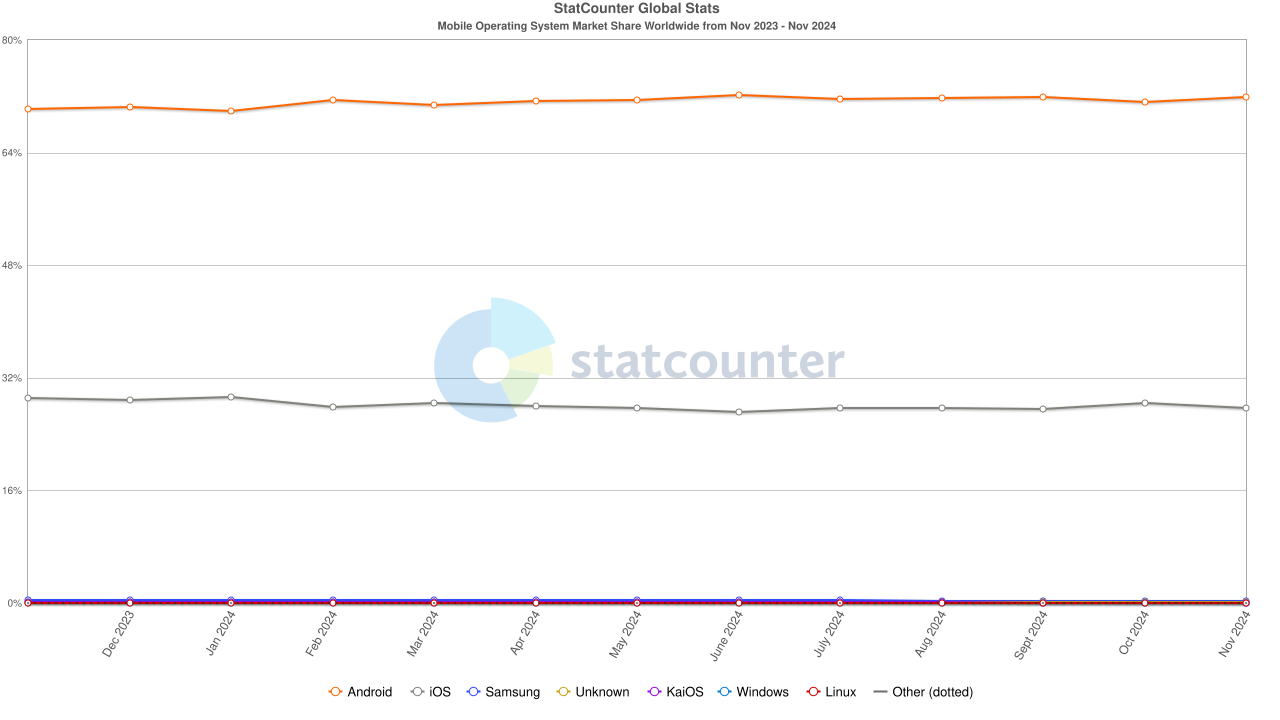
\includegraphics[width=0.8\textwidth]{2024全球智能手机市场占有率统计.png}
    \caption{2024全球智能手机操作系统市场占有率统计}
  \end{figure}
Android作为Google公司开发的开源操作系统,其在国内市场也有广泛的应用领域,滋养了移动端设备的蓬勃发展。但是中美科技战的背景下,
高端移动设备的芯片进口受到限制,产业发展受制于人。龙芯作为国产自主芯片的领头羊,于2021年推出了自主指令集Loongson Architecture(LoongArch)[2],
涵盖基础架构、虚拟化、向量指令等多个部分。将安卓移植到龙芯指令集上不仅有利于丰富完善龙芯的软件生态,而且会为后续的移动端国产化替代提供一个探索性的方案。

Android 系统作为主流的移动操作系统,其图形栈的设计与实现不仅影响了应用程序的性能,还直接关系到用户的整机体验。
Android 图形栈的复杂性体现在其多层架构中,包括应用层、框架层、硬件抽象层(HAL)及底层驱动。
这种多层结构使得开发者能够灵活地利用不同的图形 API,如 OpenGL ES 和 Vulkan,以实现高效的图形渲染。
随着技术的发展,越来越多的应用程序对图形处理的需求不断增加,尤其是在游戏、虚拟现实(VR)和增强现实(AR)等领域。

尽管 Android 图形栈在设计上具有高度的灵活性和可扩展性,但在实际应用中仍面临诸多挑战。例如,不同设备的硬件差异使得图形性能的优化变得复杂。
这使得开发者需要针对不同设备进行优化,以确保应用在各种硬件上的流畅运行。
此外,Android 的多任务处理机制可能导致图形渲染时的资源竞争,进而影响应用的响应速度和帧率。这一问题在资源密集型应用中尤为明显,
如大型游戏或复杂的图形应用。研究表明,游戏应用中的帧率波动会直接影响用户的留存率,帧率是影响用户满意度的关键因素[3]。

为了解决这些问题,研究者和开发者可以采取多种优化策略。通过合理使用缓存和减少绘制调用,可以显著提升图形渲染的效率。例如,
使用纹理和图形对象的重用能够减少 GPU 的负担,从而提高帧率。此外,利用 Android 提供的性能分析工具,如 Systrace 和 GPU Profiler,
可以帮助开发者识别性能瓶颈,进行针对性的优化。

通过对图形栈的研究和优化,可以提高应用程序的图形渲染效率,加快界面的响应速度,降低卡顿现象的发生频率。此外
一个稳定的图形栈可以减少应用程序崩溃和系统崩溃的可能性,提高系统的稳定性和可靠性,保障
用户数据的安全性;优化应用程序的图形渲染流程,提高应用程序的性能表现,减少资源占用,降
低功耗消耗,从而提升开发效率和节约开发成本。因此,对 Android 图形栈的研究具有重要的理论和实际意义。

% 随着应用程序对图形性能和视觉效果要求的提高,Android 图形栈面临着诸多挑战。
% 首先,移动设备的硬件资源有限,如何在有限的内存和处理能力下实现高效的图形渲染成为关键问题。
% 其次,随着 3D 游戏和高分辨率视频内容的普及,图形栈需要支持更复杂的渲染技术和算法。
% 此外,Android 设备的多样性使得跨设备优化和兼容性问题变得尤为重要。

% 近年来,Vulkan API 的引入为 Android 图形栈提供了新的发展方向。Vulkan 作为一种低开销、高性能的图形 API,
% 允许开发者更细粒度地控制 GPU 资源,提升渲染性能。对 Vulkan 的深入研究有助于理解其在 Android 图形栈中的应用及优化。

% 对 Android 图形栈的研究不仅具有学术价值,还有重要的实际意义:

% 1.提升用户体验:通过优化图形渲染流程和算法,能够显著提高应用的响应速度和图形质量,为用户提供更加流畅和生动的视觉体验。

% 2.推动技术创新:研究图形栈中的新技术(如 Vulkan、机器学习在图形处理中的应用等)能够推动整个行业的技术进步,
% 促进新一代移动应用的发展。

% 3.优化资源管理:理解 Android 图形栈的工作机制,能够帮助开发者更高效地管理资源,提高应用的性能和稳定性,
% 降低能耗,延长设备的使用寿命。

% 4.助力开发者工具的完善:深入研究图形栈的各个组成部分,有助于开发更好的开发者工具和框架,简化开发流程,提高开发效率。

\section{国内外研究现状}
\subsection{移动端显卡驱动现状}
1.移动设备显卡驱动
移动设备显卡驱动用于处理智能手机、平板电脑和其他移动设备的图形渲染任务。与桌面显卡驱动相比,它们在功耗和散热方面的优化尤为重要,
以确保设备的电池寿命和用户体验。移动显卡驱动的主要功能有实现低功耗优化,动态调整 GPU 的频率和电压,以节约电池电量;
图形加速,支持高效的 2D/3D 渲染,以提高用户界面和应用程序的图形性能;视频解码和编码,为高清视频和流媒体播放提供硬件加速支持;
以及高效的图形API支持,移动驱动通常支持 OpenGL ES 和 Vulkan,以实现高效的图形渲染。常见的移动设备的显卡驱动有ARM Mali驱动,
Qualcomm Adreno 驱动,Imagination PowerVR 驱动,苹果 A 系列和 M 系列芯片。

1.ARM Mali驱动:ARM Mali驱动是为ARM Mali GPU设计的一套图形处理单元驱动程序,它支持OpenGL ES、Vulkan、OpenCL等图形和计算接口,
用于嵌入式设备和移动设备的图形处理。Mali GPU广泛应用于智能手机、平板电脑、智能电视和其他嵌入式系统。已有多个GPU系列产品的配套驱动,如
Utgard、Midgard、Bifrost、Valhall等,同时有开源和闭源的驱动实现,开源实现由Panfrost、Lima等社区开发,
而闭源实现则是由ARM 官方提供的 Mali GPU 驱动。

2.Qualcomm Adreno 驱动:Qualcomm Adreno 是高通公司为其 Snapdragon 系列芯片设计的 GPU(图形处理单元),
广泛应用于智能手机、平板电脑和其他嵌入式设备。Adreno 驱动程序为这些设备提供图形渲染和计算能力,
支持现代图形 API(如 OpenGL ES、Vulkan 和 OpenCL),用于运行复杂的图形和计算任务。
如同Mali驱动一样,Adreno也有开源和闭源的实现。freedreno 是 Linux 社区开发的开源 Adreno 驱动,支持 OpenGL ES 和 Vulkan。
闭源实现是由Qualcomm 提供,通常嵌入到 Android 中,提供完整的 GPU 功能支持和性能优化。

3.Imagination PowerVR 驱动:应用于Imagination Technologies 的 PowerVR 系列 GPU,用以支持高效图形和计算解决方案以及
延迟渲染架构(Deferred Rendering Architecture),并且提供提供高效的渲染性能和低功耗的特性。该驱动被用于许多移动设备,
如部分 iPhone 和其他手机品牌。通常是闭源的,优化只针对特定硬件。

4.苹果 A 系列和 M 系列芯片:适用于苹果自研的苹果的 A 系列和 M 系列芯片,A 系列主要用于 iPhone 和 iPad,
M 系列则主要用于 Mac 和 iPad,二者都基于 ARM 架构设计。该驱动程序针对苹果的硬件进行深度优化,
以提供高性能、低功耗的图形处理能力。


% 关键技术:Tiling 渲染:移动 GPU 驱动经常使用 tile-based 渲染架构来减少带宽需求和功耗。
% 异步计算:驱动程序支持异步任务,以提高图形渲染和计算任务的并行处理能力。
% 热管理:驱动程序会监控设备温度,并动态调整性能以防止过热。

% 图形模拟器?
% x11
% mesa
% gpu模拟器:gpgpu sim
% 命令队列 commandqueue

\subsection{安卓显示应用层的优化}
Google的优化:由于安卓图形栈的性能与用户体验高相关,Google 本身也在对图形栈做一些优化。Android 4.1
之后,Google 对 Android Display 系统进行了重构,实现了黄油工程(Project Butter),在系统受到
VSync pulse 后,马上开始下一帧的渲染,称为 drawing with VSync,让 CPU/GPU 有完整的时间来处
理数据,减少了卡顿(jank),具体实现上引入了 Choreographer[6]。在 Android 7.0 版本之后,首次
引入 Vulkan API,实现了低开销和高性能的特点,并且允许多线程同时提交工作到 GPU。相比较
OpenGL ES,Vulkan 在性能提升、帧率提升、cpu 使用率等方面均有较大提升。在Android 9.0 版本中,引入了
minigbm,旨在为 Android 提供更灵活的缓冲区管理,并用一种标准化的方式来管理和分配图形缓冲区,与 
Direct Rendering Manager(DRM)紧密结合,使得在 Linux 设备上进行图形输出和显示变得更加高效,满足了
嵌入式设备对性能和资源管理的严格要求。

补充内容:
张超等[6]实现了SurfaceFlinger在桌面Linux的X Window环境下运行。其主要方法是通过替换gralloc硬件模块使用Linux上的窗口引擎,
也就是使用软件渲染的方式将SurfaceFlinger合成的图像写入共享内存,
 再由一个桌面图形程序输出画面. 该方法的不足是使用软件渲染而没有调用GPU实现硬件加速, 造成占用大量CPU时间, 并且画面输出过程需要不断调用IPC,
 在处理3D图形时只有个位数的帧数, 性能较为低下。
\begin{figure}[h]
  \centering
  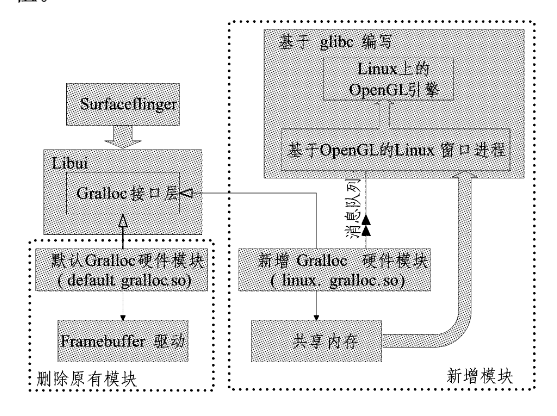
\includegraphics[width=0.8\textwidth]{Android图形系统向桌面Linux的移植.png}
  \caption{Android图形系统向桌面Linux的移植}
\end{figure}

Android X86[5]项目使用Mesa的OpenGL ES实现,成功运行了可在X86架构下运行硬件加速的SurfaceFLinger。江帆[4]提出了一种可以在X Window系统下运行Android SurfaceFlinger的方案,并且可以使用硬件加速。
\section{研究内容与挑战}

\subsection{难点与挑战}
\subsection{工作贡献与创新}

\section{本文的组织架构}
本文第一章时绪论部分,介绍研究背景和意义,国内外研究现状,并对全文的组织结构进行阐述。

第二章围绕课题介绍了安卓图形显示的原理和相关技术,包括安卓图形系统个部分组件,如何构建安卓系统以及内核的支持等。以及龙芯
平台提供的底层支持如GPU以及固件等。

第三章着重分析安卓图形系统的整体结构,以及分析如何在龙芯平台上运行安卓图形,包括分析渲染和加载龙芯驱动的关键流程,所需的各个组件支持,以及为了适应
龙芯硬件平台所必须做的一些调整

第四章是性能分析和优化,暂定。。。

第五章是对整个图形系统包括龙芯专有驱动在内的实现进行评估和测试,包括测试环境,功能测试,性能测试等。

第六章对论文的工作内容作了总结,分析了所构建系统的优势与不足,并对课题的未来研究方向做出了一些展望和建议。

